\section{Basic Concepts}
\subsection{Quantum bits (qubits)}

Classical bits: $0, 1$ \newline
Quantum bit \textit{qubit}: Superposition of $0$ and $1$:

A quantum state $\ket{\psi}$ is described as 
\begin{equation}
    \ket{\psi} := \alpha \ket{0} + \beta \ket{1}, \quad \alpha, \beta \in \mathbb{C} 
\end{equation}
where 
\begin{equation}
    \abs{\alpha}^2 + \abs{\beta}^2 = 1 \quad \text(normalization).
\end{equation}
%
Mathematical description: $\ket{\psi} \in \mathbb{C}^2$ with
\begin{equation*}
    \ket{0} = \begin{pmatrix}1 \\ 0 \end{pmatrix}, 
    \quad \ket{1} = \begin{pmatrix}0 \\ 1\end{pmatrix}
    \quad \leadsto \ket{\psi} = \begin{pmatrix}
        \alpha \\ \beta
    \end{pmatrix}
\end{equation*}


Different from classical bits, cannot (in general) directly observe / measure a qubit 
(the amplitudes $\alpha$ and $\beta$).
%
Instead: "\textit{standard}" measurement will result in 
\begin{itemize}
    \item $0$ with probability $\abs{\alpha}^2$
    \item $1$ with probability $\abs{\beta}^2$
\end{itemize}
%

The measurement also \underline{changes} the qubit (\textit{wavefunction collapse}).
%
If measuring $0$, the qubit will be $\ket{\psi} = \ket{0}$ directly after the measurement,
and likewise if measuring $1$, the qubit will be $\ket{\psi} = \ket{1}$. \newline

In practise: Can estimate the probabilities $\abs{\alpha}^2$ and $\abs{\beta}^2$ in 
experiments by repeating the same experiment many times (i.e via outcome statistics).
These repetitions are called \textit{trials} or \textit{shots}.

\begin{figure}[h]
    \centering
    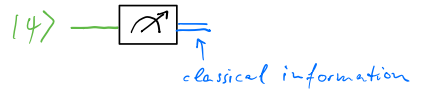
\includegraphics[scale=0.5]{chapters/res/circuit-notation.png}
    \caption{Circuit notation}
\end{figure}
\newpage

A useful graphical deputation of a qubit is the \underline{Bloch sphere} representation:
If $\alpha$ and $\beta$ happen to be real-valued, then can find angle 
$\vartheta \in \mathbb{R}$ such that
\begin{equation}
    \alpha = \cos{\frac{\vartheta}{2}}, \quad \beta = \sin{\frac{\vartheta}{2}}
\end{equation}
\begin{equation*}
    (\leadsto \abs{\alpha}^2 + \abs{\beta}^2 
    = \cos{\frac{\vartheta}{2}} + \sin{\frac{\vartheta}{2}}) = 1 \quad \color{green}\checkmark
\end{equation*}

\begin{figure}[h]
    \centering
    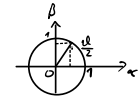
\includegraphics[scale=0.5]{chapters/res/bloch_sphere_sin_cos.png}
\end{figure}

In general: represent 
\begin{align*}
    \alpha &= e^{i \gamma} \cos{\frac{\vartheta}{2}} \\
    \beta &= e^{i (\varphi + \gamma)} \sin{\frac{\vartheta}{2}} \\
\end{align*}
using so-called phase angles $\gamma$ for $\alpha$ and $\varphi + \gamma$ for $\beta$.

\begin{figure}[h]
    \centering
    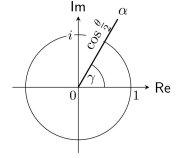
\includegraphics[scale=0.6]{chapters/res/sin-cos-complex.png}
\end{figure}

Then:
\begin{align}
    \ket{\psi} &= 
        e^{i \psi} \cos{\frac{\vartheta}{2}} \cdot \ket{0} 
        + \underbrace{e^{i (\varphi + \gamma)}}_{= \text{ } e^{i\varphi} \cdot e^{i\gamma}} \sin{\frac{\vartheta}{2}} \cdot \ket{1} \\
        %
        &= \underbrace{e^{i \gamma}}_{\text{can be ignored here}}
        \left(\cos{\frac{\vartheta}{2}} \cdot \ket{0} + e^{i\varphi} \cdot \sin{\frac{\vartheta}{2}} \cdot \ket{1}\right)
\end{align}

Thus $\ket{\psi}$ is characterized by two angles $\varphi$ and $\gamma$;
these specify the point defined as 
\begin{equation*}
    \vec{r} = \begin{pmatrix}
        \cos{\varphi} \cdot \sin{\vartheta} \\
        \sin{\varphi} \cdot \cos{\vartheta} \\
        \cos{\vartheta}
    \end{pmatrix}
\end{equation*}

on the surface of a sphere:
\begin{figure}[h!]
    \centering
    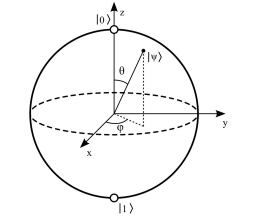
\includegraphics[scale=0.5]{chapters/res/bloch-sphere.png}
    \caption{Bloch Sphere (Felix Bloch)}
\end{figure}

\subsection{Single qubit gates}

Principles of \underline{time evolution}: The quantum state $\ket{\psi}$ at current
time point $t$ transitions to a new quantum state $\ket{\psi'}$ at a later time point
$t' > t$. \newline
Transition described by a complex unitary matrix $U$:
\begin{equation}
    \ket{\psi'} = U \cdot \ket{\psi}
\end{equation}

\begin{figure}[h!]
    \centering
    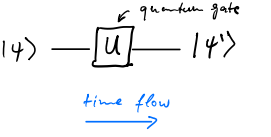
\includegraphics[scale=0.5]{chapters/res/circuit_time_evolution.png}
    \caption{Circuit notation}
\end{figure}

Notes: 
\begin{itemize}
    \item Circuit is read from left to right, but matrix times vector ($U\ket{\psi}$) from right to left.
    \item $U$ preserves normalization
\end{itemize}

Examples:
\begin{itemize}
    \item Quantum analogue of the classical NOT gate ($0 \leftrightarrow 1$) flip
    $\ket{0} \leftrightarrow \ket{1}$ leads to Pauli-X gate:
    \begin{equation}
        X \equiv \sigma_1 = \begin{pmatrix}
            0 & 1 \\
            1 & 0
        \end{pmatrix}
    \end{equation}

    Check: $X\ket{0} = \begin{pmatrix}
            0 & 1 \\
            1 & 0
        \end{pmatrix} \begin{pmatrix}0 \\ 1 \end{pmatrix} = \ket{1}$ and 
        $X\ket{1} = \begin{pmatrix}
            0 & 1 \\
            1 & 0
        \end{pmatrix} \begin{pmatrix}1 \\ 0 \end{pmatrix} = \ket{0} 
        \quad \color{green}\checkmark $
    
    \item Pauli-Y gate: 
    \begin{equation}
        Y \equiv \sigma_2 = \begin{pmatrix}
            0 & -i \\
            i & 0
        \end{pmatrix}
    \end{equation}

    \item Pauli-Z gate: 
    \begin{equation}
        Z \equiv \sigma_3 = \begin{pmatrix}
            1 & 0 \\
            0 & -1
        \end{pmatrix}
    \end{equation}

    Z leaves $\ket{0}$ unchanged, but flips the sign of the coefficient of $\ket{1}$.
    Recall the Bloch Sphere representation:
    \begin{equation*}
        \ket{\psi} = \cos{\frac{\vartheta}{2}} \cdot \ket{0} + e^{i\varphi} \sin{\frac{\vartheta}{2}} \cdot \ket{1}
    \end{equation*} 

    Then
    \begin{align*}
        Z \ket{\psi} &= \cos{\frac{\vartheta}{2}} \cdot \ket{0} {\color{red}\text{ }-\text{ }}
            e^{i\varphi} \sin{\frac{\vartheta}{2}} \cdot \ket{1} \\
        %
        &\stackrel{e^{i\pi} = -1}{=} \cos{\frac{\vartheta}{2}} \cdot \ket{0} + 
            \underbrace{e^{i\pi} e^{i\varphi}}_{e^{i(\varphi + \pi)}} \sin{\frac{\vartheta}{2}} \cdot \ket{1}
    \end{align*}

    $\leadsto$ new Bloch Sphere angles: $\vartheta' = \vartheta, \varphi = \varphi + \pi$ 
    (rotating by $\pi = 180^\circ$ around z-axis) \newline
    X, Y, Z gates are called \underline{Pauli matrices}.
    The \underline{Pauli vector} $\vec{\sigma} = (\sigma_1, \sigma_2, \sigma_3) = (X, Y, Z)$
    is a vector of $2 \times 2$ matrices.

    \item Hadamard Gate:
    \begin{equation*}
        H = \frac{1}{\sqrt{2}}  \begin{pmatrix}
            1 & 1 \\
            1 & -1
        \end{pmatrix}
    \end{equation*}

    \begin{figure}[h]
        \centering
        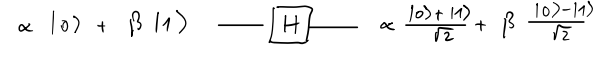
\includegraphics[scale=0.5]{chapters/res/hadamard-gate-circuit.png}
        \caption{Hadamard Gate}
    \end{figure}

    \item Phase Gate:
    \begin{equation*}
        S = \begin{pmatrix}
            1 & 0 \\
            0 & i
        \end{pmatrix}
    \end{equation*}

    \item T Gate:
    \begin{equation*}
        T = \begin{pmatrix}
            1 & 0 \\
            0 & e^{i\pi/4}
        \end{pmatrix}
    \end{equation*}
    Note: $T^2 = S$ since $(e^{i \pi /4})^2 = e^{i\pi/2} = i$
\end{itemize}


Pauli matrices satisfy:
\begin{enumerate}
    \item $\sigma^{2}_{j} = I$ (identifity) for $j = 1,2,3$
    \item $\sigma_j \cdot \sigma_k = - \sigma_k \sigma_j$ for all $j \neq k$
    \item ${\color{blue} [} \sigma_j, \sigma_k {\color{blue} ]} :=
        \underbrace{\sigma_j \sigma_k - \sigma_k \sigma_j}_{\text{Commutator}} = 
        2 i \sigma_l$ for $(j,k,l)$ a cyclic permutation of (1,2,3).
\end{enumerate}

General definition of \underline{matrix exponential}

\begin{equation}
    exp(A) \equiv e^A = \sum_{k = 0}^{\infty} \frac{1}{k!}A^k, \quad A \in \mathbb{C}^{n \times n}
\end{equation}

Special case: $A^2 = I, x \in \mathbb{R}$
\begin{align*}
    e^{i A x} &= \underbrace{\sum_{k = 0}^{\infty} \frac{1}{(2k)!} (ix)^{2k} 
        \underbrace{A^{2k}}_{(A^2)^k = I^k = I}}_\text{even} +
        \underbrace{\sum_{k = 0}^{\infty} \frac{1}{(2k + 1)!} (ix)^{2k + 1} 
            \underbrace{A^{2k+1}}_{(A^2)^k \cdot A = I^k \cdot A= A}}_\text{odd} \\
        &= \underbrace{\sum_{k = 0}^{\infty} \frac{1}{(2k)!} (-1)^k x^{2k}}_{ = \cos{x}} \cdot I +
        \underbrace{\sum_{k = 0}^{\infty} \frac{1}{(2k + 1)!} (-1)^k x^{2k + 1}}_{=i \sin{x}} \cdot A\\
        &= \cos{x} \cdot I + i \sin{x} A
\end{align*}
(generalizes Euler's formula $e^{ix} = \cos{x} + i \sin{x}$)
\newline

This can be used to define the following \underline{rotation operators} via the
Pali matrices. Let $\vartheta \in \mathbb{R}$:

\begin{align}
    R_x(\vartheta) &:= e^{-i \vartheta X / 2} 
        = \cos{\frac{\vartheta}{2}} I - i \sin{\frac{\vartheta}{2}} X 
        = \begin{pmatrix}
            \cos{\frac{\vartheta}{2}} & -i \sin{\frac{\vartheta}{2}} \\
            -i \sin{\frac{\vartheta}{2}} & \cos{\frac{\vartheta}{2}}
        \end{pmatrix} \\
    %
    R_y(\vartheta) &:= e^{-i \vartheta Y / 2} 
        = \cos{\frac{\vartheta}{2}} I - i \sin{\frac{\vartheta}{2}} Y 
        = \begin{pmatrix}
            \cos{\frac{\vartheta}{2}} & -\sin{\frac{\vartheta}{2}} \\
            \sin{\frac{\vartheta}{2}} & \cos{\frac{\vartheta}{2}}
        \end{pmatrix} \\ 
    R_z(\vartheta) &:= e^{-i \vartheta Z / 2} 
        = \cos{\frac{\vartheta}{2}} I - i \sin{\frac{\vartheta}{2}} Z
        = \begin{pmatrix}
            e^{-i \vartheta / 2} & 0 \\
            0 & e^{i \vartheta / 2}
        \end{pmatrix}
\end{align} 
\newpage


General case: Rotation about an axis $\vec{v} \in \mathbb{R}^3$
(normalized such that $\norm{\vec{v}}) = \sqrt{v_1^2 + v_2^2 + v_3^3} = 1$): \newline
using the notation:

\begin{equation}
    \braket{\vec{v}}{\vec{\sigma}} 
        = \vec{v} \cdot \vec{\sigma} 
        = v_1 \sigma_1 + v_2 \sigma_2 + v_3 \sigma_3
        = \begin{pmatrix}
            v_3 && v_1 - i v_2 \\
            v_1 + i v_2 && -v_3
        \end{pmatrix}
\end{equation}

It holds that $(\vec{v} \cdot \vec{\sigma})^2 = I$.

We define the rotation operator around axis $\vec{v}$ as 
\begin{equation}
    R_v(\vartheta) := e^{-i \vartheta (\vec{v} \cdot \vec{\sigma}) / 2} 
        = \cos{\frac{\vartheta}{2}} I - i \sin{\frac{\vartheta}{2}} (\vec{v} \cdot \vec{\sigma})
\end{equation}

Note: $R_x$, $R_y$, $R_z$ are special cases corresponding to $\vec{v} = (1, 0, 0)$, 
$\vec{v} = (0, 1, 0)$, and $\vec{v} = (0, 0, 1)$. \newline 

Can derive that the Bloch Sphere representaiton of $R_{\vec{v}}(\vartheta)$ 
is a "conventional" rotation (in three dimensions) by angle $\vartheta$ about 
axis $\vec{v}$.

\begin{figure}[h]
    \centering
    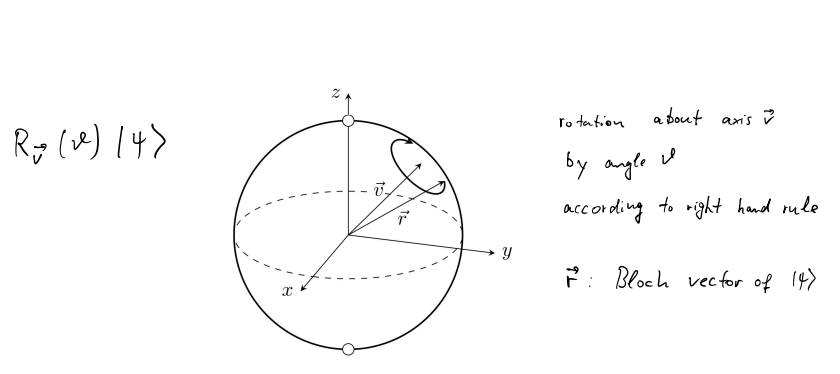
\includegraphics[scale=0.5]{chapters/res/bloch-sphere-rotation.png}
    \caption{Circuit notation}
\end{figure}


\underline{Z-Y decomposition} of an arbitrary $2 \times 2$ unitary matrix: \newline
For any unitary matrix $U \in \mathbb{C}^{n \times n}$ there exist real numbers
$\alpha, \beta, \gamma, \delta \in \mathbb{R}$ such that

\begin{equation}
    U = e^{i \alpha} \underbrace{\begin{pmatrix}
        e^{-i \beta / 2} & 0 \\
        0 & e^{i \beta / 2} 
    \end{pmatrix}}_{R_z(\beta)} \cdot 
    \underbrace{\begin{pmatrix}
        \cos{\frac{\gamma}{2}} & -\sin{\frac{\gamma}{2}} \\
        \sin{\frac{\gamma}{2}} & \cos{\frac{\gamma}{2}}
    \end{pmatrix}}_{R_y(\gamma)} \cdot 
    \underbrace{\begin{pmatrix}
        e^{-i \delta / 2} & 0 \\
        0 & e^{i \delta / 2} 
    \end{pmatrix}}_{R_z(\delta)}
\end{equation}

\subsection{Multiple qubits}